\section{Zielsetzung}
\label{sec:Zielsetzung}

In diesem Versuch soll die Suszeptibilität von Oxiden einiger Seltener-Erd-Elemente näher untersucht und anschließend die Ergebnisse mit den theoretischen Werte verglichen werden.

\section{Theorie}
\label{sec:Theorie}
\subsection{Berechnung der Suszeptibilität}
\label{subsec: Berechnung}
Für die magnetische Flussdichte $\vec{B}$ und die magnetische Feldstärke $\vec{H}$ im Vakuum gilt 
\begin{equation}
\label{eq:eq1}
\vec{B} = \mu_0 \vec{H}
\end{equation}
wobei $\mu_0$ die Induktionskonstante ist. Die Flussdichte hängt unter anderem auch von der Magnetisierung $\vec{M}$ der im Feld vorhandener Materialien ab. Die Magnetisierung $\vec{M}$ wird auch unter anderem durch magnetische Momente hervorgerufen und hängt von der magnetischen Feldstärke $\vec{H}$ ab.
Die Gleichung \ref{eq:eq1} wird ergänzt durch die Magnetisierung $\vec{M}$ und es gilt:
\begin{equation}
\label{eq:eq2}
\vec{B} = \mu_0 \vec{H} + \vec{M}.
\end{equation}
Für die Magnetisierung wird die folgende Beziehung gegeben:
\begin{equation}
\vec{M} = \mu_0 \chi \vec{H}
\end{equation}
die dann in der Gleichung \ref{eq:eq2} eingesetzt wird und schließlich ergibt sich:
\begin{equation*}
\vec{B} = \mu_0 \vec{H} + \mu_0 \chi \vec{H}
\end{equation*}
wobei die Größe $\chi$ die sogenannte Suszeptibilität ist. Die Suszeptibilität ist eine materialabhängige Größe, die zusätzlich von der Temperatur und der Feldstärke abhängen kann. 

Das hier betrachtete Phänomen des Paramagnetismus entsteht nicht bei jedem Material und ist nicht bei jedem Material zu beobachten. Dieser wird nur bei solchen Materialien beobachtet, deren Drehimpuls nicht verschwinden kann. Es entsteht in Materialien deren Atome einen magnetischen Moment zu einem äußeren Feld besitzen. Der Paramagnetismus ist temperaturabhängig, weil die Orientierung der magnetischen Momente durch die thermische Bewegung der Atome dauerhaft geändert wird.

Im Folgenden soll ein Zusammenhang zwischen dem Drehimpuls und dem magnetischen Moment betrachtet werden. 
Der Gesamtdrehimpuls $\vec{J}$ ist eine quantenmechanische Größe, die mit dem Gesamtdrehimpuls der Elektronen und deren Spins zusammenhängt, wobei dieser hier vernachlässigt wird. 
Es folgt nun:
\begin{equation*}
\vec{J} = \vec{L} + \vec{S},
\end{equation*}
wobei $\vec{L}$ und $\vec{S}$ die Vektorsumme der Einzeldrehimpulse der Elektronen sind. Aus der Quantenmechanik ergibt sich:
\begin{align*}
\vec{\mu_\text{L}} &= -\frac{\mu_\text{B}}{\hbar}\vec{L} \\
\vec{\mu_\text{S}} &= -g_\text{S}\frac{\mu_\text{B}}{\hbar}\vec{S} 
\end{align*}
wobei $\mu_\text{B}$ das Bohrsche Magneton und $g_\text{S}$ das gyromagnetische Verhältnis sind. 
\begin{figure}[h!]
	\centering
	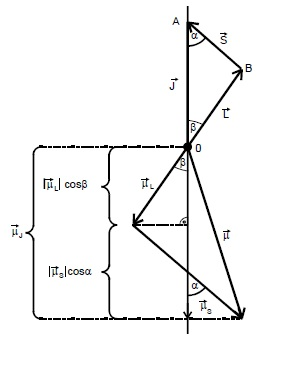
\includegraphics[width=0.6\linewidth]{Vektordarstellung.jpg}
	\caption{Vektordarstellung der Drehimpulse in einer Elektronenhülle und der magnetischen Momente, \cite[3]{anleitung606}.}
	\label{fig:vektordarstellung}
\end{figure}

In diesem Fall werden die Beträge der magnetischen Momente betrachtet und mit Hilfe der Beziehung:
\begin{equation*}
\left|\vec{J}\right| = \sqrt{J(J+1)}\hbar,
\end{equation*}
die bei den anderen Drehimpulsen auch analog gilt, ergeben sich die folgenden Ausdrücke für die magnetischen Momente:
\begin{align}
\label{eq:eq3}
\left|\vec{\mu_\text{L}}\right| &= \mu_\text{B}\sqrt{L(L+1)} \\
\left|\vec{\mu_\text{S}}\right| &= g_\text{S}\mu_\text{B}\sqrt{S(S+1)}.
\end{align}
Mit Hilfe der Beziehung aus den Gleichungen \ref{eq:eq3} und aus der Abbildung \ref{fig:vektordarstellung} ergibt sich der folgende Ausdruck für $\left|\vec{\mu_\text{J}}\right|$:
\begin{equation*}
\left|\vec{\mu_\text{J}}\right| = \left|\vec{\mu_\text{S}}\right|\text{cos}\alpha + \left|\vec{\mu_\text{L}}\right|\text{cos}\beta.
\end{equation*}
Es wird angenommen, dass das gyromagnetische Verhältnis den Wert $2$ hat. Mit dieser Näherung lässt sich das magnetische Moment des Gesamtdrehimpulses zu:
\begin{equation}
\label{eq:eq4}
\left|\vec{\mu_\text{J}}\right| \approx \mu_\text{B} \sqrt{J(J+1)} \frac{3J(J+1)+S(S+1)-L(L+1)}{2J(J+1)}
\end{equation}
vereinfachen. Aus der Gleichung \ref{eq:eq4} wird der letzte Teilausdruck:
\begin{equation}
g_\text{J} = \frac{3J(J+1)+S(S+1)-L(L+1)}{2J(J+1)}
\label{eqn:lande}
\end{equation}
als Land\'{e}-Faktor bezeichnet. Ein weiteres Phänomen der Quantenmechanik ist die Richtungsquantelung. Die Richtungsquantelung ist die Tatsache, dass der Winkel zwischen einer beliebigen gewählten Richtung des äußeren Feldes und der Lage von $\left|\vec{\mu_\text{J}}\right|$ nicht beliebig sein kann. Es gilt für die Z-Komponente der folgende Ausdruck:
\begin{equation}
\label{eq:eq5}
\mu_{\text{J}_\text{Z}} = - \mu_\text{B}g_\text{J}m
\end{equation}
wobei $m$ die Orientierungsquantenzahl ist. Der Winkel kann daher nur $2J+1$ Einstellungsmöglichkeiten annehmen. Für jede mögliche Einstellung wird eine potentielle Energie angegeben, mit welcher die Magnetisierung $\vec{M}$ bestimmt werden kann. Die potentielle Energie ist gegeben als:
\begin{equation*}
E_\text{m} = - \vec{\mu_\text{J}}\vec{B} = \mu_\text{B}g_\text{J}mB.
\end{equation*}
Die Aufspaltung der Spektrallinien in $2J+1$ unter dem Einfluss eines äußeren Magnetfeldes wird als $\mathit{Zeeman-Effekt}$ bezeichnet. Hier muss die Häufigkeit der bestimmten Orientierungen des magnetischen Momente berechnet werden, diese mit dem Betrag des zugehörigen magnetischen Momentes aus der Gleichung \ref{eq:eq5} multizipliert und anschließend über alle vorkommende Orientierungen summiert. Mit verschiedenen Näherungen und quantenmechanischen Betrachtungen lässt sich ein Ausdruck für $\chi$ herleiten.

Das sogenannte $\mathit{Curie-Gesetz}$ lautet:
\begin{equation}
\label{eq:mariecurie}
\chi = \frac{\mu_0\mu_\text{B}^{2}g_\text{J}^{2}NJ(J+1)}{3kT}
\end{equation}
wobei $k$ die Boltzmann-Konstante, $T$ die Temperatur und $N$ die Anzahl der Momente pro Volumeneinheit sind. Für hohe Temperaturen ist die Suszeptibilität $\chi$ proportional zu $\frac{1}{T}$.

Der Paramagnetismus wird insbesondere bei Ionen Seltener Erden beobachtet, die durch $4$f-Elektronen entstehen. Aus der Gleichung \ref{eq:mariecurie} lässt sich erschließen, dass die inneren Elektronen große Drehimpulse besitzen. Um die Anordnung der Elektronen in der $4$f-Schale und der sich daraus ergebende Gesamtdrehimpuls zu verstehen, werden die Hundschen Regeln einige Erklärungen dafür liefern. 

$\blacktriangleright$ Der Gesamtspin $\vec{S}$ nimmt den maximal möglichen Wert an, die Spins der einzelnen Elektronen $\vec{s_\text{i}}$ stehen also möglichst parallel. 

$\blacktriangleright$ Wenn eine Schale höchstens zur Hälfte gefüllt ist, dann ist der Gesamtdrehimpuls $\vec{J} = \vec{L} - \vec{S}$, bei mehr als die Hälfte ist es umgekehrt, $\vec{J} = \vec{L} + \vec{S}$.

$\blacktriangleright$ Der Drehimpuls $\vec{L} = \sum \vec{l_\text{i}}$ nimmt die größtmögliche Summe an, wenn die Bahndrehimpulse $\vec{l_\text{i}}$ unter Berücksichtigung des Pauli-Prinzips und der ersten Regel bilden können.

\subsection{Messung der Suszeptibilität}
\begin{figure}[h!]
	\centering
	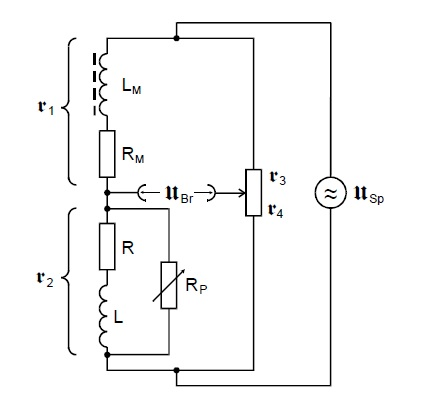
\includegraphics[width=0.7\linewidth]{bruckenschaltung.jpg}
	\caption{Brückenschaltung für die Messung der Suszeptibilität, \cite[8]{anleitung606}.}
	\label{fig:bruckenschaltung}
\end{figure}
Für die tatsächliche Messung von $\chi$ wird eine Brückenschaltung wie in der Abbildung \ref{fig:bruckenschaltung} mit zwei Induktivitäten benutzt. Mithilfe der Schaltung wird die Induktivität der Spule gemessen in der das zu untersuchende Material liegt.

Aus der Induktivität wird die Suszeptibilität $\chi$ bestimmt:
\begin{equation}
\label{eq:indu}
L_\text{M} = \mu_0 \frac{n^2F}{l} + \chi \mu_0 \frac{n^2Q}{l}
\end{equation}
wobei $n$ die Windungszahl, $l$ die Länge, $F$ den Querschnitt der Spule und $Q$ die Querschnittfläche der Probe sind. Der letzte Term in der Gleichung \ref{eq:indu} ist Induktivitätsdifferenz $\Delta L$ zwischen materiegefüllten und Luftspulen. Zur Messung der Suszeptibilität $\chi$ gibt es zwei verschiedene Methoden. Zum einen wird die Brücke abgeglichen und die zu gehörende Spule mit dem zu untersuchenden Material der Suszeptibilität $\chi$ gefüllt, so kann die Suszeptibilität $\chi$ aus der Brückenschaltung errechnet werden. Die Brückenspannung ergibt sich nach Kirchhoff zu:
\begin{equation*}
U_\text{Br} = \frac{r_1r_4-r_3r_2}{(r_1+r_2)(r_3+r_4)}U_\text{Sp}.
\end{equation*}
Es folgt direkt die Abgleichsbedingung für die Brückenspannung:
\begin{equation*}
r_1r_4 = r_3r_2.
\end{equation*}
Der Widerstand $r_1$ ist bedingt durch die Induktion der Spule durch:
\begin{equation*}
r_1 = R_\text{M} + j \omega L_\text{M}.
\end{equation*}
Mit der Näherung $R_\text{p} \gg R $ und $R_\text{p} \gg \omega L$ ergibt sich $r_2$ zu:
\begin{equation*}
r_2 \approx R + j \omega L.
\end{equation*}
Für sehr hohe Frequenzen $\omega^2 L^2 \gg R^2$ wird die Suszeptibilität nach mehreren Näherungen und Umformungen vereinfacht zu:
\begin{equation}
\chi(\omega \rightarrow \infty) = 4 \frac{F}{Q}\frac{U_\text{Br}}{U_\text{Sp}}
\end{equation}
wobei $U_\text{Sp}$ die Speisespannung ist.
Zum anderen wird nach dem Abgleichen der Brücke die Spule mit Material gefüllt und die Brücke erneut abgeglichen.
Der Widerstand $r_3$ muss also angepasst werden um wieder eine ausgeglichene Brücke zu erhalten:
\begin{equation*}
r_3' = r_3 + \Delta r.
\end{equation*}
Aus den neuen Angleichsbedingungen ergibt sich die folgende Formel:
\begin{equation}
\chi = 2 \frac{\Delta R}{R_3}\frac{F}{Q}
\label{eqn:chiwiderstand}
\end{equation}
wobei $R_3$ der Widerstand am Potentiometer ist und $\Delta R$ die Differenz der Einstellungen an diesem.